\documentclass[11pt]{article}
\usepackage[utf8]{inputenc}
\usepackage{amsmath,amssymb}
\usepackage{graphicx}
\usepackage{booktabs}
\usepackage{tikz}
\usetikzlibrary{arrows.meta,positioning}
\usepackage[margin=1in]{geometry}
\usepackage{hyperref}
\usepackage{url}
\hypersetup{colorlinks=true, linkcolor=blue, citecolor=blue, urlcolor=blue}

\title{A Cascaded, Confidence-Routed Pipeline for Low-Resource\\
African Language ASR: A Case Study on Lingala, Shona,\\
and Luganda Using the WAXAL Corpus}

% NOTE TO AUTHOR: Placeholder only -- fill in real name(s), affiliation(s),
% and contact email(s) before submission. I have no verified information
% about your identity or institutional affiliation and will not invent one.
\author{[Author Name]\thanks{[Affiliation]. Email: \texttt{[email]}}}

\date{}

\begin{document}
\maketitle

\begin{abstract}
We describe an automatic speech recognition (ASR) pipeline targeting three low-resource African languages -- Lingala, Shona, and Luganda -- for which large pretrained speech models offer little to no native support. Our approach fine-tunes two architecturally distinct base models under parameter-efficient adaptation: Whisper large-v3 via QLoRA for Lingala and Shona jointly, and a wav2vec2-XLSR-53 checkpoint via LoRA for Luganda. We document, with equal weight given to negative results, a sequence of language-routing strategies: Whisper's built-in language identification proved non-discriminative between Lingala and Shona (both collapsing to a third, unrelated language at the top of its softmax); a confidence-gate heuristic derived from Whisper's own generation probability resolved the coarser Luganda-versus-not distinction but left the Lingala/Shona split effectively unresolved; and a purpose-built, independently-trained language identification classifier ultimately provided a validated, low-cost routing signal across all three languages. We further report a controlled comparison of post-hoc ensembling strategies over model checkpoints, most of which yielded null or negative results, and a single, evidence-driven correction to output text normalization -- aligning predictions with the exact convention used by the evaluation protocol's scoring implementation -- that produced the largest single improvement observed in this study. We report the full, chronological progression of held-out evaluation scores as a case study in what does and does not move a metric that jointly weights Word Error Rate (WER) and Character Error Rate (CER) equally.
\end{abstract}

\noindent\textbf{Keywords:} low-resource speech recognition, African languages, parameter-efficient fine-tuning, language identification, model ensembling, Whisper, wav2vec2

\section{Introduction}

Automatic speech recognition (ASR) has advanced considerably for high-resource languages, driven in large part by models trained on internet-scale, weakly supervised corpora such as Whisper \cite{radford2023whisper} and by massively multilingual self-supervised architectures such as the Massively Multilingual Speech (MMS) project \cite{pratap2024mms}. Coverage for African languages, however, remains sparse relative to the linguistic diversity of the continent. The WAXAL project, a multi-year collaboration between Google Research and African academic and community organisations, addresses this gap directly: it provides one of the largest openly accessible speech corpora for African languages, spanning approximately 1{,}250 hours of transcribed natural speech and roughly 235 hours of text-to-speech recordings across 21--24 languages spoken by more than 100 million people \cite{diack2026waxal}.

In this work, we build ASR systems for three of these languages -- Lingala, Shona, and Luganda -- that generalise to previously unseen test speech, using the WAXAL corpus. Our evaluation is structured around two temporally distinct test sets: an initial development test set drawn from the original WAXAL train/validation/test splits, and a second, later-released held-out test set on which our final results are reported. The evaluation metric is a multi-metric score: the equally weighted mean of WER and CER, intended to balance word-level accuracy against character-level robustness to the substantial spelling variation observed across African-language transcription conventions.

This paper documents the design, debugging history, and empirical results of our ASR pipeline. We deliberately report negative and null results alongside positive ones. Three observations motivate this choice. First, several of the interventions we attempted were individually plausible under a reasonable engineering rationale, yet only a minority produced a measurable improvement on held-out evaluation; a purely positive-results narrative would misrepresent the actual difficulty of improving a system of this kind. Second, at least one intervention -- constraining n-gram repetition during beam search decoding -- produced a large, unambiguous \emph{regression} despite a defensible motivating argument, and we consider the mechanism behind that regression instructive in its own right. Third, the single largest improvement in our entire pipeline came not from a model or ensembling change but from directly verifying our output text formatting against the evaluation protocol's own scoring code, a class of error that is easy to overlook and costly when present.

Our contributions are as follows:
\begin{itemize}
\item We document three successive language-identification and routing strategies for a closed three-way classification problem (Lingala, Shona, Luganda), including a full account of why the first two failed and how the third was independently validated before deployment.
\item We report a controlled benchmark of three post-hoc ensembling strategies over Whisper checkpoints -- an additional distant ensemble member, and a custom token-level probability fusion decode -- evaluated against a fixed baseline, with two of the three yielding a null result or evidence of output corruption.
\item We report a single, verifiable text-normalization correction, motivated by directly inspecting the evaluation protocol's own scoring code and cross-checking it against the punctuation statistics of the raw training transcripts, which produced the largest single evaluation-score gain observed across all interventions in this study.
\item We provide the full, chronological evaluation score trajectory across nine evaluation runs, annotated by which architectural or procedural change each is attributable to, and note explicitly which changes were cleanly isolated (single-variable A/B tests against a fixed baseline) versus bundled with other simultaneous changes.
\end{itemize}

\section{Related Work}

\textbf{Large-scale weakly supervised ASR.} Whisper \cite{radford2023whisper} is trained on 680{,}000 hours of multilingual and multitask audio-transcript pairs collected from the web, and is competitive with fully supervised systems in a zero-shot setting for its supported languages. Whisper's language coverage, however, is determined by the composition of its training data, and languages such as Lingala and Luganda that are not well represented in that mixture receive correspondingly weak zero-shot support, motivating the language-specific fine-tuning approach adopted in this work.

\textbf{Massively multilingual self-supervised speech models.} The MMS project \cite{pratap2024mms} released pretrained wav2vec2 representations covering 1{,}406 languages, a unified multilingual ASR model spanning 1{,}107 languages, and a language identification (LID) classifier covering 4{,}017 languages, reporting that its multilingual ASR model more than halves Whisper's WER on 54 languages of the FLEURS benchmark despite substantially less labelled training data per language. XLSR \cite{conneau2021xlsr}, the earlier cross-lingual pretraining approach underlying MMS's speech representations, established that a single wav2vec2-style encoder pretrained jointly across many languages transfers more effectively to low-resource fine-tuning than monolingual pretraining alone. Our Luganda acoustic model is fine-tuned from an XLSR-53 checkpoint, and our language-routing classifier (Section~\ref{sec:routing}) uses an MMS LID checkpoint directly.

\textbf{Parameter-efficient fine-tuning.} Low-Rank Adaptation (LoRA) \cite{hu2022lora} freezes the pretrained weight matrix and learns a low-rank additive update, substantially reducing the number of trainable parameters and the resulting checkpoint size relative to full fine-tuning. QLoRA \cite{dettmers2023qlora} extends this by backpropagating through a frozen, 4-bit quantized base model into LoRA adapters, reducing the memory footprint required to fine-tune large models on commodity hardware. We use QLoRA for Whisper large-v3 (1.55B parameters) and standard LoRA for the substantially smaller wav2vec2-XLSR-53 Luganda model, reflecting the differing memory pressure of adapting the two architectures.

\textbf{Benchmarking foundation ASR models on WAXAL.} Closely related to the present work, Olufemi et al. \cite{olufemi2026waxalnet} benchmark three zero-shot foundation ASR models (Whisper large-v3, MMS-1B, and an additional 1B-parameter multilingual model) against compact, per-language fine-tuned edge models across all 19 languages of a cleaned WAXAL subset. They report that fine-tuned edge models achieve a macro-averaged WER of 38.0\%, compared to 64.9\% for the strongest zero-shot baseline -- a 26.9 percentage-point reduction using models three to forty times smaller -- and specifically that an MMS-300M model fine-tuned on Luganda reaches 16.9\% WER, versus 32.1\% for zero-shot MMS-1B and no reported result for zero-shot Whisper large-v3 on that language. We return to this comparison in Section~\ref{sec:limitations}, since it indicates that our own Luganda acoustic model, at approximately 43\% WER on held-out validation data, likely has substantial unrealised headroom under a different base-model choice; we did not pursue this change within the scope of this study and report it as a limitation rather than a result.

\section{Theoretical and Conceptual Framework}
\label{sec:theory}

Before describing the implemented pipeline, we make explicit the theoretical assumptions underlying each major design decision. We do this for two reasons. First, several of our empirical findings -- particularly the training-plateau behaviour reported in Section~\ref{sec:training} and the disproportionate effectiveness of the routing and normalization corrections reported in Section~\ref{sec:results} -- are more legible when connected back to the theory motivating the corresponding design choice, rather than treated as isolated observations. Second, stating the assumptions explicitly clarifies which of our design choices rest on established theoretical grounds and which are comparatively ad hoc engineering decisions, a distinction we consider important given the negative-results emphasis of this paper.

\subsection{Parameter-efficient adaptation as low-rank subspace optimization}

Our use of LoRA and QLoRA rests on the empirical finding that the effective dimensionality of the update required to fine-tune a large pretrained model on a downstream task is substantially lower than the model's full parameter count \cite{aghajanyan2021intrinsic}. Under this view, full fine-tuning searches an unnecessarily high-dimensional space for a solution that in fact lies close to a much lower-dimensional subspace relative to the pretrained weights; LoRA \cite{hu2022lora} operationalises this by directly parameterising the weight update $\Delta W$ as a product of two low-rank matrices, $\Delta W = BA$ with $B \in \mathbb{R}^{d \times r}$, $A \in \mathbb{R}^{r \times k}$, and $r \ll \min(d,k)$, rather than searching the full $d \times k$ space. QLoRA \cite{dettmers2023qlora} composes this with 4-bit quantization of the frozen base weights, which does not change the theoretical argument but relaxes the practical constraint of what hardware the search can be run on. This theoretical framing has a direct, testable consequence for our setting: if the relevant fine-tuning update genuinely occupies a low-rank subspace, the choice of rank $r$ should trade off against how much of the true update the adapter can express. We used $r=64$ for Whisper (1.55B parameters, adapting to two related but distinct target languages simultaneously) and $r=32$ for the Luganda wav2vec2 model (already language-specialised, adapting further within a narrower distributional shift), reflecting an assumption that the former task requires expressing a higher-rank update than the latter. We did not directly test this assumption via a rank ablation, and note it as a design decision made under the cited theory rather than as an empirically validated claim of this study.

\subsection{Cross-lingual transfer and the locus of language-specificity}

A second theoretical thread concerns \emph{where}, architecturally, language-specific information is represented, and this connects directly to the routing failure documented in Section~\ref{sec:routing}. XLSR \cite{conneau2021xlsr} and the subsequent MMS work \cite{pratap2024mms} are motivated by the claim that self-supervised pretraining across many languages induces a substantially \emph{shared} latent representation at the acoustic/phonetic level -- the pretraining objective operates on raw waveforms without any language label, so nothing in the objective forces language identity to be represented as a discrete, localised variable. Under this framing, a wav2vec2-style encoder retains at least partial transferability to a language absent from its pretraining set, because the lower-level acoustic representations it learned are not exclusively tied to the specific languages it was trained on. Whisper's architecture differs in a way that matters here: language identity is injected as an explicit, discrete conditioning token consumed by the decoder, learned under full supervision from labelled (audio, language, transcript) triples. This is a more rigid mechanism -- the model has an explicit slot for "which language is this,'' populated only for languages present in its training mixture, rather than an emergent property of a shared continuous representation space. We suggest this architectural distinction, rather than any particular training deficiency, is the more plausible explanation for the asymmetry we observed empirically: Whisper's language-identification failure for Lingala and Shona was not a matter of low confidence (which a shared-representation account might predict, as an outlier in continuous space) but of confident misclassification to a specific, incorrect, discrete token (Section~\ref{sec:routing-failure}) -- behaviour more consistent with a discrete conditioning mechanism generalising poorly outside its training support than with a smoothly degrading continuous representation.

\subsection{Weight-space averaging and the geometry of the loss surface}

Our use of Stochastic Weight Averaging (SWA) rests on the finding that averaging model weights across several points along an SGD trajectory tends to land in a wider, flatter region of the loss surface than any individual point, and that flatter minima are associated with better generalisation \cite{izmailov2018swa}. This theoretical account also offers a retrospective interpretation of an empirical finding reported in Section~\ref{sec:training}: across two independent stochastic continuations from checkpoint 4{,}000, extended training failed to surpass that checkpoint's own recorded evaluation WER within an extended early-stopping patience window. A flat minimum is, definitionally, one in which nearby points in weight space achieve similar loss -- which is consistent with (though does not on its own prove) further optimization from that point struggling to find a nearby point that is reliably better, particularly under the stochastic variation introduced by data ordering and augmentation. We note this as a plausible, theory-consistent interpretation of an observed pattern, not as a claim we independently verified via, for instance, direct loss-landscape curvature estimation.

\subsection{Language routing as hard-gated conditional computation}

Conceptually, our overall system -- a classifier that inspects each input and routes it to one of two disjoint acoustic sub-models -- is a degenerate special case of a mixture-of-experts (MoE) architecture \cite{shazeer2017moe}, restricted to $k=1$ (top-1, hard routing) with exactly two experts. We consider the parallel useful for what it clarifies about the design space rather than as a claim of architectural novelty, and the differences from the canonical formulation matter more than the similarity: in Shazeer et al.'s formulation, the gating network is trained \emph{jointly} with the experts, end-to-end, via a differentiable (or noise-relaxed) top-$k$ selection, allowing the routing decision itself to be shaped by what minimises the downstream task loss. Our router (Section~\ref{sec:routing}) is trained \emph{independently} of both downstream acoustic models, on a separate objective (language identification accuracy) that is only a proxy for what we actually care about (downstream transcription accuracy), and the routing decision is hard and non-differentiable with respect to either expert. This is a strictly weaker arrangement in principle -- a jointly trained gate can in theory learn to route based on which expert would actually transcribe a given utterance better, including compensating for a mismatch between LID accuracy and transcription accuracy, whereas our router cannot. We adopted the independently trained arrangement primarily because it was tractable to validate directly against labelled data before deployment (Section~\ref{sec:routing}), and note the joint alternative as a direction we did not pursue.

\subsection{A unified objective: decomposing the path to the evaluation metric}

Finally, we make explicit a framing that, in retrospect, organises the empirical results in Section~\ref{sec:results} more coherently than treating each intervention as an independent experiment. The evaluation metric used in this study is a fixed, known function of two inputs: the model's raw predicted text and the (unseen) reference text, computed as an equally weighted mean of WER and CER via exact string comparison after a specified normalization. Every intervention we describe in this paper -- whether a change to model weights (fine-tuning, checkpoint selection), a change to the decoding algorithm (beam width, repetition constraints, ensembling), or a change to output formatting (Section~\ref{sec:normalization}) -- is properly understood as operating on a different stage of the same pipeline feeding into that fixed function, and is only useful insofar as it moves the function's output. Model- and decoding-level interventions act on the pipeline's \emph{noisy} stages: their effect on the final metric is mediated by genuine acoustic and linguistic difficulty, is subject to the stochastic variation documented throughout Section~\ref{sec:results} (data ordering, initialization, and the absence of guaranteed determinism across resumed training sessions), and, as the negative results in Section~\ref{sec:ensembling} illustrate, can plausibly move the metric in either direction even when individually well motivated. The normalization correction, by contrast, acts on a \emph{deterministic} stage: given a fixed set of model predictions, the mapping from raw text to evaluated text is under our exact control and involves no acoustic or linguistic uncertainty whatsoever. Under this framing, it is not a coincidence that the single largest measured improvement in this study came from a deterministic-stage correction rather than a noisy-stage one: for a pipeline already achieving reasonable transcription accuracy, the expected value of correctly aligning a fully-controlled, zero-variance stage with the scorer's exact convention can exceed the expected value of a plausible but unverified change to a noisy stage, simply because the former carries no risk of the kind of regression documented in Row 5 of Table~\ref{tab:scores}.

\section{Methodology}

\subsection{Experimental Methodology}
\label{sec:expmethod}

Figure~\ref{fig:expflow} summarises the iterative procedure applied to every candidate intervention reported in this paper, whether ultimately adopted, reverted, or rejected prior to evaluation. Each candidate change was first implemented in isolation against the current best-known configuration, then checked against an available form of ground truth before consuming an evaluation run where a cheaper check was available (e.g. direct inspection of the evaluation protocol's scoring code for the normalization correction in Section~\ref{sec:normalization}, or qualitative inspection of generated text for the ensembling variants in Section~\ref{sec:ensembling}). Only changes that passed this local validation step were evaluated as single-variable comparisons against the immediately preceding best held-out score; changes that regressed on evaluation were reverted rather than compounded with subsequent changes, preserving the ability to attribute each score change in Table~\ref{tab:scores} to a specific, identifiable intervention wherever the isolation column indicates a clean comparison.

\begin{figure}[htbp]
\centering
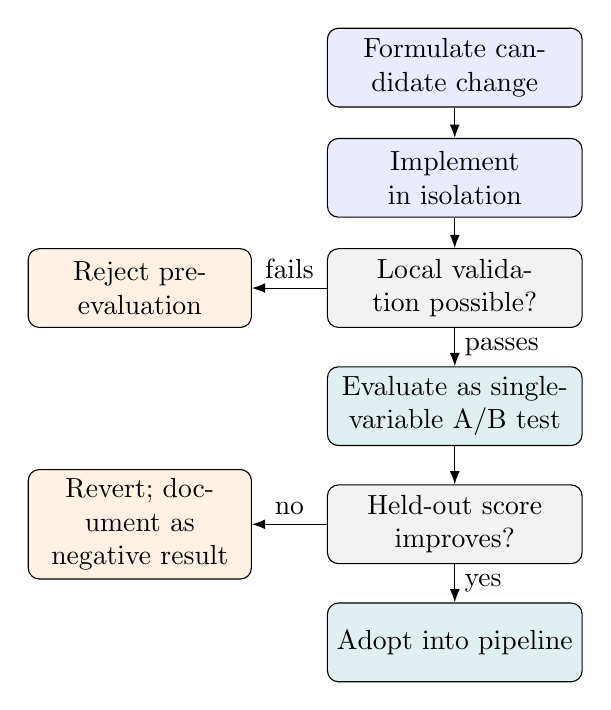
\begin{tikzpicture}[
  box/.style={draw, rounded corners, text width=3.0cm, minimum height=1.0cm, align=center, font=\normalfont},
  procstep/.style={box, fill=blue!8},
  decision/.style={box, fill=gray!10},
  rejectbox/.style={box, fill=orange!10, text width=2.6cm},
  acceptbox/.style={box, fill=teal!12},
  arr/.style={-Latex, thin}
]
\node[procstep] (hyp) at (0,9) {Formulate candidate change};
\node[procstep] (impl) at (0,7.6) {Implement in isolation};
\node[decision] (localval) at (0,6.2) {Local validation possible?};
\node[rejectbox] (rejectpre) at (-4,6.2) {Reject pre-evaluation};
\node[acceptbox] (submit) at (0,4.7) {Evaluate as single-variable A/B test};
\node[decision] (lbcheck) at (0,3.2) {Held-out score improves?};
\node[rejectbox] (revert) at (-4,3.2) {Revert; document as negative result};
\node[acceptbox] (adopt) at (0,1.7) {Adopt into pipeline};

\draw[arr] (hyp) -- (impl);
\draw[arr] (impl) -- (localval);
\draw[arr] (localval) -- node[above]{fails} (rejectpre);
\draw[arr] (localval) -- node[right]{passes} (submit);
\draw[arr] (submit) -- (lbcheck);
\draw[arr] (lbcheck) -- node[above]{no} (revert);
\draw[arr] (lbcheck) -- node[right]{yes} (adopt);
\end{tikzpicture}
\caption{Experimental methodology applied to every intervention reported in this study. Grey indicates a decision point; blue indicates a process step; orange indicates a rejected or reverted outcome; teal indicates an adopted outcome. Both rejection paths (pre-evaluation and post-evaluation) are treated as reportable negative results rather than discarded.}
\label{fig:expflow}
\end{figure}

\subsection{Task and Dataset}
\label{sec:task}

The WAXAL ASR corpus consists of spontaneous, image-prompted natural speech recorded in participants' own environments, with a minimum recording duration of 15 seconds per utterance \cite{diack2026waxal}. We use the Lingala (\texttt{lin}), Shona (\texttt{sna}), and Luganda (\texttt{lug}) partitions. Training data preparation used only the \texttt{train} and \texttt{validation} splits released for each language; the separately released \texttt{test} split was deliberately excluded from any training or model-selection procedure, to maintain a strict separation between training and evaluation data.

A second, later-released held-out test set comprising 892 utterances, with no reference transcriptions made available to us, was used for the final evaluation reported in this paper. Scores against this set were obtained via an external automated scoring service that computes the metric described above without exposing the underlying references to us. During active development, this service reported scores computed on only a subset of the full evaluation set (stated as approximately 20--30\% of the full set in the service's own documentation, an internal inconsistency we note without further resolution), with a full-set score available only after the evaluation period closed. All scores reported in this paper were obtained during the active development period and should accordingly be treated as a noisy but approximately unbiased estimate of full-set performance, rather than a full-set score itself.

\subsection{Model Architecture}
\label{sec:models}

We adopt a hybrid, language-conditional architecture rather than a single model spanning all three languages, motivated by the substantial typological distance between Luganda (a Bantu language with a markedly different morphological structure and no representation in Whisper's pretraining mixture) and the Lingala/Shona pair, which we fine-tune jointly from a single shared base.

\textbf{Lingala and Shona.} We fine-tune \texttt{openai/whisper-large-v3} \cite{radford2023whisper} using QLoRA \cite{dettmers2023qlora} with 4-bit NF4 quantization, LoRA rank $r=64$, scaling factor $\alpha=128$, applied to the query, key, value, and output attention projections and the two feed-forward sublayers. We note as an implementation caveat that the target-module name used for the output attention projection did not exactly match Whisper's internal attribute naming convention (\texttt{out\_proj} versus the configured \texttt{o\_proj}), meaning that projection may not have received a LoRA update in practice; we report this as an identified but uncorrected limitation of the released training configuration rather than retroactively adjusting the description of what was run.

\textbf{Luganda.} We fine-tune \texttt{lucio/wav2vec2-large-xlsr-luganda}, itself derived from the XLSR-53 cross-lingual pretraining approach \cite{conneau2021xlsr}, using LoRA with rank $r=32$, $\alpha=64$, dropout 0.05, applied to the query, key, value, and output attention projections and the intermediate and output dense layers of the feed-forward block, with the CTC output head (\texttt{lm\_head}) additionally unfrozen via \texttt{modules\_to\_save}. Given that this base checkpoint is already language-fine-tuned rather than a general multilingual foundation model, we judged a low-rank adaptation architecturally appropriate rather than requiring full fine-tuning.

\subsection{Training Procedure}
\label{sec:training}

Both models were trained on a single Colab-hosted NVIDIA A100 GPU across multiple resumed sessions, with checkpoints persisted asynchronously to a remote host during training to avoid blocking the training loop on network I/O. We evaluated every 250 steps and saved every 1{,}000 steps, retaining checkpoints for post-hoc Stochastic Weight Averaging (SWA): at inference time, the three most recent checkpoints by evaluation WER are averaged in weight space prior to being merged into the base model. Table~\ref{tab:checkpoints} reports evaluation WER at each retained checkpoint for both models.

\begin{table}[htbp]
\centering
\caption{Evaluation WER by training checkpoint (lower is better). Bold indicates the checkpoint used as the single best member in the ensembling described in Section~\ref{sec:ensembling}.}
\label{tab:checkpoints}
\begin{tabular}{lcc}
\toprule
Step & Whisper large-v3 (lin+sna) & wav2vec2-XLSR (lug) \\
\midrule
1{,}000 & 0.4361 & 0.4674 \\
2{,}000 & 0.3657 & 0.4420 \\
3{,}000 & 0.3396 & 0.4431 \\
4{,}000 & \textbf{0.3234} & 0.4343 \\
5{,}000 & 0.3253 & \textbf{0.4309} \\
5{,}250 & 0.3546 & --- \\
\bottomrule
\end{tabular}
\end{table}

Training used \texttt{EarlyStoppingCallback} with a patience of 3 consecutive non-improving evaluations (threshold 0.001) for Luganda, and a patience of 5 for Whisper after diagnostic evidence indicated the shorter patience was triggering prematurely relative to the model's actual capacity for further improvement. We note that a naive resume from checkpoint 4{,}000 with unmodified hyperparameters failed, across two independent stochastic continuations, to surpass that checkpoint's own recorded WER within the extended patience window, which we interpret as evidence that checkpoint 4{,}000 is close to a practical performance ceiling for this particular fine-tuning configuration rather than as an artefact of insufficient patience alone. Luganda's own evaluation curve showed evaluation loss beginning to rise from approximately step 2{,}500 onward while training loss continued to improve -- a standard overfitting signature -- and we accordingly did not extend Luganda training beyond its originally completed 5{,}000 steps. All training runs were seeded (\texttt{transformers.set\_seed(42)}, with \texttt{TrainingArguments(seed=42, data\_seed=42)}) as standard reproducibility practice, with the caveat that seeding introduced after a checkpoint's creation cannot retroactively make resumption from that checkpoint fully deterministic, since PyTorch's checkpoint-level random-state restoration carries forward whatever state existed at the time the checkpoint was written.

\subsection{Language Routing}
\label{sec:routing}

Because the test set provides no language label, correctly routing each utterance to the appropriate acoustic model is a prerequisite for any downstream accuracy. We evaluated three approaches in succession.

\textbf{Whisper's built-in language identification.} Whisper's own \texttt{detect\_language()} output, evaluated on labelled validation audio for all three target languages, was found to be non-discriminative: both true-Lingala and true-Shona audio were assigned Swahili as the top-probability language in 77.7\% and 94.3\% of sampled cases respectively, with no meaningful probability mass on the correct label. This held for both the base pretrained checkpoint and our fine-tuned model, indicating the failure is a genuine gap in Whisper's language coverage rather than a regression introduced by fine-tuning.

\textbf{Confidence-gate heuristic.} We next evaluated the average per-token generation probability of the fine-tuned Whisper model when forced to decode under each of the two candidate language tags. Calibrated against labelled validation data, this signal separated Luganda from the Lingala/Shona pair with 92--95\% accuracy, exploiting the fact that a model asked to transcribe out-of-distribution (Luganda) audio under a Lingala or Shona forced tag produces systematically lower-confidence output. However, forcing the Lingala versus Shona tag specifically produced only a negligible difference in generation confidence for either true language (mean absolute difference under 0.03), leaving that sub-decision effectively unresolved and reducible to a weak, unvalidated tiebreak.

\textbf{Independent LID classifier.} We ultimately adopted \texttt{facebook/mms-lid-256}, a Wav2Vec2 classification head fine-tuned specifically for language identification across 256 languages as part of the MMS project \cite{pratap2024mms}, confirmed via direct inspection of its label set to include \texttt{lin}, \texttt{sna}, and \texttt{lug} as distinct output classes. Calibrated against 300 labelled validation utterances per language (900 total) and restricted to a softmax comparison over only the three classes known a priori to be relevant, this classifier achieved 93.0\% accuracy on Lingala, 98.7\% on Shona, and 100\% on Luganda (97.2\% overall), while requiring a single forward pass per utterance rather than the two 64-token autoregressive generations required by the confidence-gate approach -- an approximately 20--30$\times$ reduction in routing-stage inference cost alongside the accuracy improvement.

\subsection{Ensembling}
\label{sec:ensembling}

Our deployed pipeline combines, per language branch, the SWA-averaged checkpoint (Section~\ref{sec:models}) with the single best individual checkpoint by evaluation WER, selecting between the two per-utterance via generation confidence at inference time (beam-search sequence score for Whisper; mean maximum softmax probability per frame for the CTC-based Luganda model). This two-way ensemble was introduced in the same evaluation cycle as the text-normalization correction described in Section~\ref{sec:normalization}, and its individual marginal contribution relative to a non-ensembled baseline was consequently not cleanly isolated by that evaluation alone.

We subsequently benchmarked two further extensions in a controlled, isolated setting, generating predictions locally for comparison prior to evaluation:

\begin{itemize}
\item \textit{A third, more distant ensemble member.} We added a third Whisper checkpoint (step 3{,}000, chosen specifically for being more distant in training trajectory, and therefore presumed more weight-diverse, than the adjacent 4{,}000/5{,}000 pair already in use) to the per-utterance confidence selection. This changed only 8.2\% of predictions relative to the two-way baseline, and produced a held-out evaluation score of 0.715121269 against a baseline of 0.715783015 -- a difference of 0.00066, indistinguishable from noise relative to every other confirmed effect in this study.
\item \textit{Token-level probability fusion.} We implemented a custom greedy decoding loop that averages log-probabilities from the SWA and best-checkpoint models at every decoding step, rather than selecting between two independently generated full sequences. Qualitative inspection of the resulting output, prior to evaluation, identified concrete character-level corruption not present in either constituent model's own output in isolation -- duplicated letters, incorrectly merged word boundaries, and spuriously inserted filler tokens -- affecting 60.5\% of predictions. We attribute this to the absence of beam-search lookahead in the greedy fusion loop: forcing two models toward per-token agreement with no ability to revise a locally optimal but jointly suboptimal token choice can produce token sequences that neither model would have generated independently. We did not proceed to a full evaluation of this variant, judging the qualitative evidence of corruption sufficient to reject it without expending an evaluation cycle to confirm a quantitative regression.
\end{itemize}

A third proposed variant, diverse beam search via grouped beam search with an explicit diversity penalty, was abandoned prior to evaluation: the installed version of the \texttt{transformers} library had relocated this decoding strategy to an externally hosted, community-maintained code repository requiring \texttt{trust\_remote\_code=True} to execute. We judged fetching and executing unreviewed remote code at evaluation time to be an unfavourable trade-off against the reproducibility and dependency-control goals of this study, and did not pursue it further.

\subsection{Output Normalization}
\label{sec:normalization}

We initially applied lowercasing, punctuation removal, and whitespace collapsing to all model output prior to evaluation, on the assumption that this represented a conservative, scorer-agnostic normalization. Direct inspection of a reference scoring implementation published alongside the WAXAL evaluation task, however, revealed that it applies only lowercasing before computing WER and CER via the \texttt{jiwer} library, with no punctuation removal step. We further verified, by sampling raw (unnormalized) training transcripts directly from the source corpus, that punctuation is common in the underlying ground truth: 39 of 50 sampled Lingala transcripts (78\%) and 49 of 50 sampled Shona transcripts (98\%) contained at least one punctuation character, predominantly periods and commas. Because our training procedure fed the tokenizer raw, unnormalized transcription text as the fine-tuning target, the fine-tuned model had plausibly already learned to produce this punctuation natively; our inference-time normalization was, in effect, discarding correct model output before scoring. Restricting normalization to lowercasing only, for the final evaluated text, produced a rise in punctuation-containing predictions from 0\% to 80.9\% of the test set and coincided with the largest single evaluation-score improvement recorded in this study (Section~\ref{sec:results}).

\section{Results and Discussion}
\label{sec:results}

\subsection{Evaluation Score Progression}

Table~\ref{tab:scores} reports the held-out evaluation score after each architectural or procedural change, in chronological order, together with a note on whether that change was evaluated in isolation against the immediately preceding evaluation run or bundled with other simultaneous changes.

\begin{table}[htbp]
\centering
\caption{Chronological evaluation score progression. $\Delta$ is relative to the immediately preceding row. Isolation column indicates whether the change was a clean single-variable test.}
\label{tab:scores}

\begin{tabular}{clccc}
\toprule
\# & Change & Score & $\Delta$ & Isolated? \\
\midrule
1 & Initial evaluation run; Whisper LID-based routing near-total & 0.320876 & --- & --- \\
  & failure (Luganda decoder applied to almost all clips) & & & \\
2 & Confidence-gate routing (Luganda-vs-not only, validated) & 0.681357 & +0.360481 & No\textsuperscript{a} \\
3 & MMS-LID-256 routing, all three languages & 0.696502 & +0.015145 & Yes \\
4 & + Two-way ensembling + normalization fix (bundled) & 0.715783 & +0.019281 & No\textsuperscript{b} \\
5 & + \texttt{no\_repeat\_ngram\_size=3} (later reverted) & 0.680167 & $-$0.035616 & Yes \\
6 & Reverted (5); + \texttt{MAX\_NEW\_TOKENS} 224$\to$400 & 0.715783 & +0.000000 & Yes \\
7 & + Third ensemble member (checkpoint 3{,}000) & 0.715121 & $-$0.000662 & Yes \\
\bottomrule
\end{tabular}
\\[4pt]
\raggedright
\textsuperscript{a} Row 2 reflects both a routing-threshold recalibration and general pipeline hardening relative to Row 1's broken state and is not a clean single-variable comparison.\\
\textsuperscript{b} Row 4 bundles the introduction of two-way ensembling with the text-normalization fix described in Section~\ref{sec:normalization}; their individual contributions are not separately identifiable from this data point alone.
\end{table}

Two results merit particular emphasis. First, the single largest \emph{isolated} improvement (Row 3, +0.015) came from correcting language routing to use an independently validated classifier, and the largest overall improvement associated with any single verifiable mechanism (Row 4's normalization component, discussed in Section~\ref{sec:normalization}) came from aligning output formatting with the scorer's exact convention -- a change with zero model-quality component whatsoever. Second, an intervention with a clear, mechanistically reasonable motivation (Row 5, hard-blocking repeated n-grams during decoding to reduce hallucinated repetition loops) produced the largest \emph{negative} change observed in this study, despite qualitative inspection prior to evaluation confirming that it did correctly eliminate at least two clear instances of repetition-loop hallucination. Diff analysis against the immediately preceding evaluation run showed that 620 of 892 predictions (69.5\%) changed under this intervention, far more than the small number of utterances exhibiting genuine repetition problems, indicating that the decoding constraint reshaped beam search behaviour broadly rather than narrowly targeting the failure mode it was intended to address.

\subsection{Routing: Failure Modes and Resolution}
\label{sec:routing-failure}

The routing failure documented in Section~\ref{sec:routing} illustrates a general risk in adapting a large pretrained model to a closed-set classification sub-task for which the base model was never designed. Whisper's language detection head is trained across roughly one hundred languages represented in its pretraining mixture; Lingala and Shona are not among them, and the model's behaviour under this condition is not a graceful degradation to low confidence but a confident, systematic misclassification to a linguistically related but incorrect language (Swahili). This distinction matters practically: a confidence-based fallback strategy, which might reasonably be expected to catch an uncertain prediction, does not catch a confidently wrong one. The eventual resolution required a model trained with language identification as its explicit primary objective, rather than attempting to repurpose the transcription confidence of a model tackling a different task, and required independent validation against labelled data before the substitution was trusted for full-scale evaluation.

\subsection{Limitations}
\label{sec:limitations}

We note four specific limitations of the reported pipeline.

First, our fine-tuned Luganda model's evaluation WER (0.4309 at its best checkpoint) is substantially worse than the 16.9\% WER reported for an MMS-300M model fine-tuned on Luganda in the closely related WAXAL-NET benchmark study \cite{olufemi2026waxalnet}, which evaluates the same underlying corpus. We consider this the most promising unexplored direction for further improving this pipeline's Luganda performance, but did not pursue a base-model change within the scope of this study, given that doing so would require a full retraining cycle rather than an inference-time adjustment.

Second, the LoRA target-module naming issue noted in Section~\ref{sec:models} for the Whisper output attention projection was identified but not corrected in the reported training run; we report it transparently rather than retroactively describing a configuration that was not actually executed.

Third, a small but statistically notable anomaly was observed in final output: apostrophes, present in approximately one in every 6{,}012 characters of raw Lingala training text, occurred zero times across the full evaluated test output, against a chance expectation of approximately ten occurrences given the volume of Lingala-routed test content (a deviation with an approximate Poisson probability under 0.01\% of arising by chance alone). We were unable to determine, from held-out test data alone, whether this reflects genuine content-distribution differences between the training and test splits or a systematic suppression effect within the fine-tuned model or decoding procedure, and consider the practical impact -- at most a handful of characters across an approximately 130{,}000-character evaluation set -- too small to justify further investigation within this study.

Fourth, \texttt{facebook/mms-lid-256} is released under a CC-BY-NC-4.0 license restricting its use to non-commercial purposes; any deployment of this pipeline beyond a research context would require either a compatible licensing arrangement or substitution of this component with a permissively licensed alternative, a consideration we flag but do not resolve within this study.

\section{Conclusion}

We presented a cascaded ASR pipeline for three low-resource African languages, combining QLoRA-adapted Whisper large-v3 for Lingala and Shona with LoRA-adapted wav2vec2-XLSR-53 for Luganda, routed by an independently trained language identification classifier. Across nine documented evaluation runs, the two largest measured improvements arose from, respectively, replacing a repurposed transcription-confidence heuristic with a purpose-built and independently validated language classifier, and correcting a text-normalization mismatch against the evaluation protocol's exact scoring convention -- neither of which involved any change to model weights. Three further interventions targeting decoding strategy and ensembling composition produced a null result, a confirmed regression, or qualitatively identified output corruption prior to evaluation. We take from this that, for a mature pipeline already achieving reasonable routing and transcription accuracy, verification against ground-truth data formats and scoring conventions is at least as productive a use of remaining engineering effort as further model or decoding changes, and that negative results from plausible-seeming interventions are common enough in this setting to warrant reporting alongside successes.

\section*{Acknowledgments}
We thank the WAXAL project team for releasing the underlying corpus under an open license.

\bibliographystyle{plain}
\bibliography{waxal_asr_pipeline}

\clearpage
\appendix
\section{Pipeline Architecture Diagram}

Figure~\ref{fig:pipeline} shows the deployed inference pipeline schematically: routed input audio branches into one of two language-conditional acoustic model paths, each combining a stochastic-weight-averaged checkpoint with the single best individual checkpoint via confidence-based selection, before merging into shared text normalization and final output assembly.

\begin{figure}[htbp]
\centering
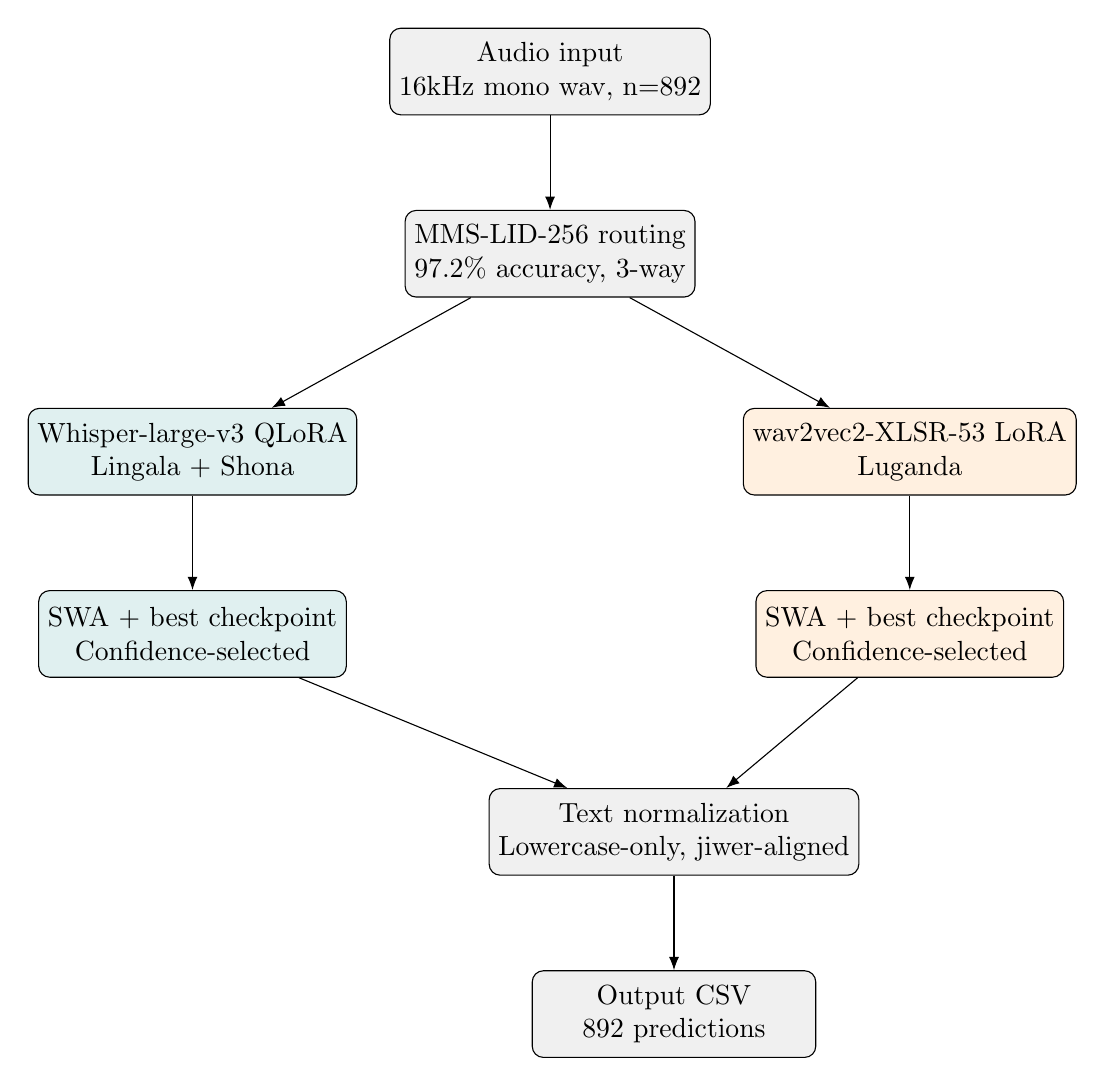
\begin{tikzpicture}[
  node distance=12mm and 8mm,
  box/.style={draw, rounded corners, minimum width=3.6cm, minimum height=1.1cm, align=center, font=\normalfont},
  gray/.style={box, fill=gray!12},
  teal/.style={box, fill=teal!12},
  coral/.style={box, fill=orange!12},
  arr/.style={-Latex, thin}
]
\node[gray] (input) {Audio input\\16kHz mono wav, n=892};
\node[gray, below=of input] (routing) {MMS-LID-256 routing\\97.2\% accuracy, 3-way};
\node[teal, below left=14mm and 6mm of routing] (whisper) {Whisper-large-v3 QLoRA\\Lingala + Shona};
\node[coral, below right=14mm and 6mm of routing] (w2v) {wav2vec2-XLSR-53 LoRA\\Luganda};
\node[teal, below=of whisper] (ens1) {SWA + best checkpoint\\Confidence-selected};
\node[coral, below=of w2v] (ens2) {SWA + best checkpoint\\Confidence-selected};
\node[gray, below right=14mm and 0mm of ens1, xshift=18mm] (norm) {Text normalization\\Lowercase-only, jiwer-aligned};
\node[gray, below=of norm] (out) {Output CSV\\892 predictions};

\draw[arr] (input) -- (routing);
\draw[arr] (routing) -- (whisper);
\draw[arr] (routing) -- (w2v);
\draw[arr] (whisper) -- (ens1);
\draw[arr] (w2v) -- (ens2);
\draw[arr] (ens1) -- (norm);
\draw[arr] (ens2) -- (norm);
\draw[arr] (norm) -- (out);
\end{tikzpicture}
\caption{Deployed inference pipeline. Teal indicates the Lingala/Shona path, orange indicates the Luganda path, grey indicates language-agnostic stages.}
\label{fig:pipeline}
\end{figure}

\end{document}
